\section{Introduction to Chemistry} \index{Chemistry! introduction}


%\section*{Importance of Chemistry}

Chemistry plays a very important role in our
daily life. Many processes at home, particularly
in the kitchen, are chemical processes we rarely
spend a day without using products from parts
of the chemical industry such as the
pharmaceutical industry, the food industry, the
paper industry and the petroleum industry to
name a few.

During an introduction to chemistry students
should be shown where their lives and the
products they use link in with the chemical
industry. Students' own experience of chemistry comes
from their daily lives and not from working in a
laboratory. A students environment is their
chemistry lab!

\begin{multicols}{2}

\subsection{Chemical Products}

\begin{center}
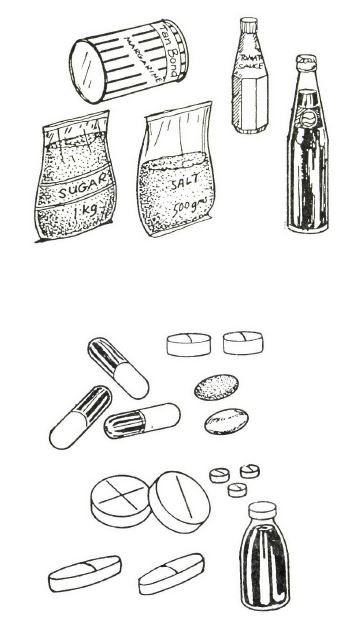
\includegraphics[width=0.46\textwidth]{./img/source/chemical-products.jpg}
\end{center}

\begin{description*}
%\item[Subtopic:]{}
%\item[Materials:]{}
%\item[Setup:]{}
\item[Procedure:]{In order to demonstrate the importance of
chemistry in daily life, ask the students to display
and label things produced by chemists. Ask
them to arrange similar products together.}
%\item[Hazards:]{}
%\item[Questions:]{}
%\item[Observations:]{}
%\item[Theory:]{}
%\item[Applications:]{}
%\item[Notes:]{}
\end{description*}

\vfill
\columnbreak


\subsection{Pollution and Chemistry} \index{Pollution}

\begin{center}
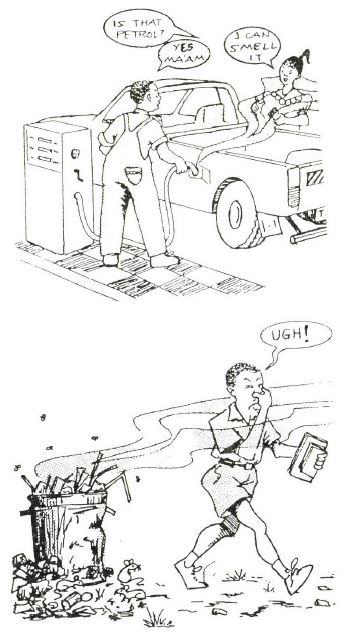
\includegraphics[width=0.45\textwidth]{./img/source/chemical-pollution.jpg}
\end{center}

\begin{description*}
%\item[Subtopic:]{}
%\item[Materials:]{}
%\item[Setup:]{}
\item[Procedure:]{In order to build up an awareness of pollution
in our environment, let the students describe
some situations where pollution of air, water
and soil happen.}
%\item[Hazards:]{}
\item[Questions:]{What can be done to reduce these forms of pollution?}
%\item[Observations:]{}
%\item[Theory:]{}
%\item[Applications:]{}
%\item[Notes:]{}
\end{description*}

\subsection{Making an Excursion}

\begin{center}
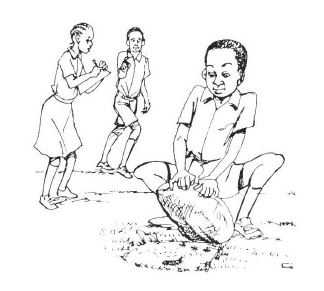
\includegraphics[width=0.45\textwidth]{./img/source/excursion.jpg}
\end{center}

\begin{description*}
%\item[Subtopic:]{}
%\item[Materials:]{}
%\item[Setup:]{}
\item[Procedure:]{It can be stimulating to make an excursion
around the school ground, to find out where
chemical processes can be observed. There can
be natural ones like the decomposition of organic
substances, cooking, alcoholic drink
production, etc.}
%\item[Hazards:]{}
%\item[Questions:]{}
%\item[Observations:]{}
%\item[Theory:]{}
%\item[Applications:]{}
%\item[Notes:]{}
\end{description*}

\subsection{Posters of Chemical Products} \index{Displays} \index{Visual aids}

\begin{center}
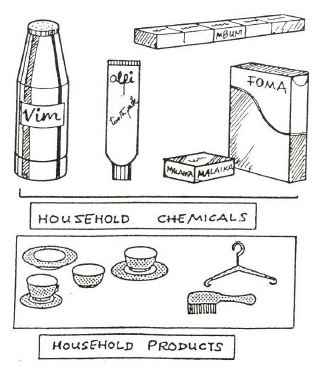
\includegraphics[width=0.45\textwidth]{./img/source/chemical-posters.jpg}
\end{center}

\begin{description*}
%\item[Subtopic:]{}
\item[Materials:]{Manila paper, marker pens, newspapers, scissors}
%\item[Setup:]{}
\item[Procedure:]{Instead of displaying real products, posters
can be made in groups with pictures cut out
from newspapers. For language training let the
pupils talk about their work and what the posters
show.}
%\item[Hazards:]{}
%\item[Questions:]{}
%\item[Observations:]{}
%\item[Theory:]{}
%\item[Applications:]{}
%\item[Notes:]{}
\end{description*}

\subsection{We Are All Chemists}

\begin{center}
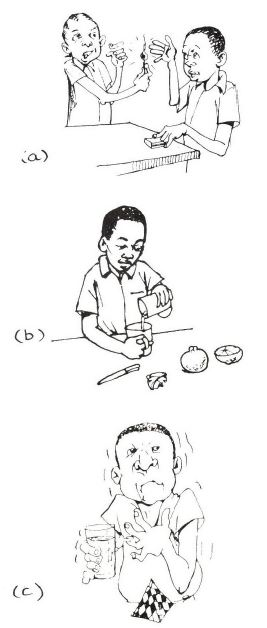
\includegraphics[width=0.45\textwidth]{./img/source/all-chemists.jpg}
\end{center}

\begin{description*}
%\item[Subtopic:]{}
%\item[Materials:]{}
%\item[Setup:]{}
\item[Procedure:]{Students should understand that we are all
chemists and not only those people working in
a chemical lab. Let them try out examples of
chemical processes with locally available
materials.
\begin{itemize}
\item[(a)] Carefully burn some paper, wood, fuel or
ignite a matchstick.
\item[(b)] Add some lemon juice to a cup of tea and
observe the colour change.
\item[(c)] Let a glass of milk go sour.
\item[(d)] Rub some red or pink petals from flowers on
wet soap firmly and observe the change of the
colour.
\item[(e)] Try to find some more examples.
\end{itemize}
}
%\item[Hazards:]{}
%\item[Questions:]{}
%\item[Observations:]{}
%\item[Theory:]{}
%\item[Applications:]{}
%\item[Notes:]{}
\end{description*}

%==================================================================================================%


\end{multicols}

\pagebreak